\chapter{Pair localization transition}

Natural first question: Does this system exhibit a localization transition? If so: what are the conserved quantities? To tackle this question, we study the level-spacing ration, the half-chain entanglement entropy of eigenstates, Thouless parameters with respect to different local observables and participation ratios with different bases.

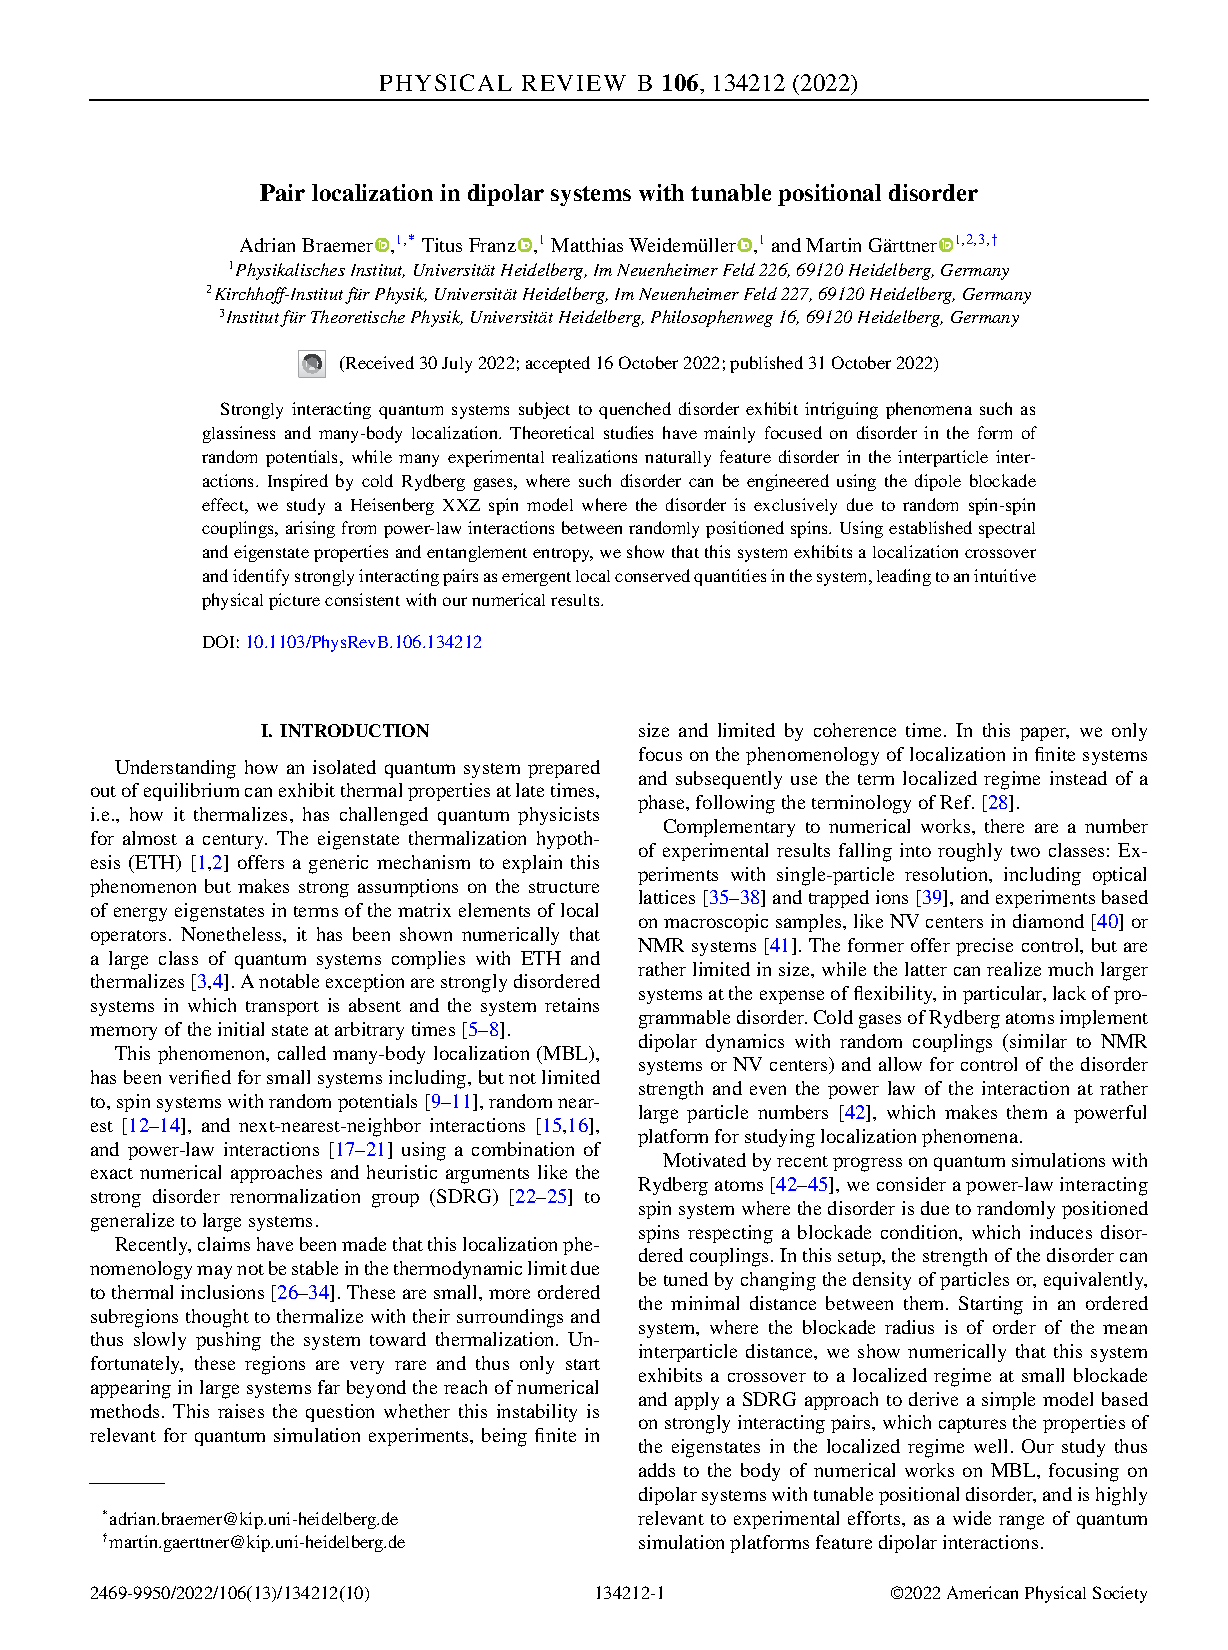
\includepdf[pages=-]{pub-Braemer2022-Pairlocalization}

\chapter{Efficient time evolution of pair localized systems}

can we exploit the knowledge about the conserved quantities to make numerics more efficient?

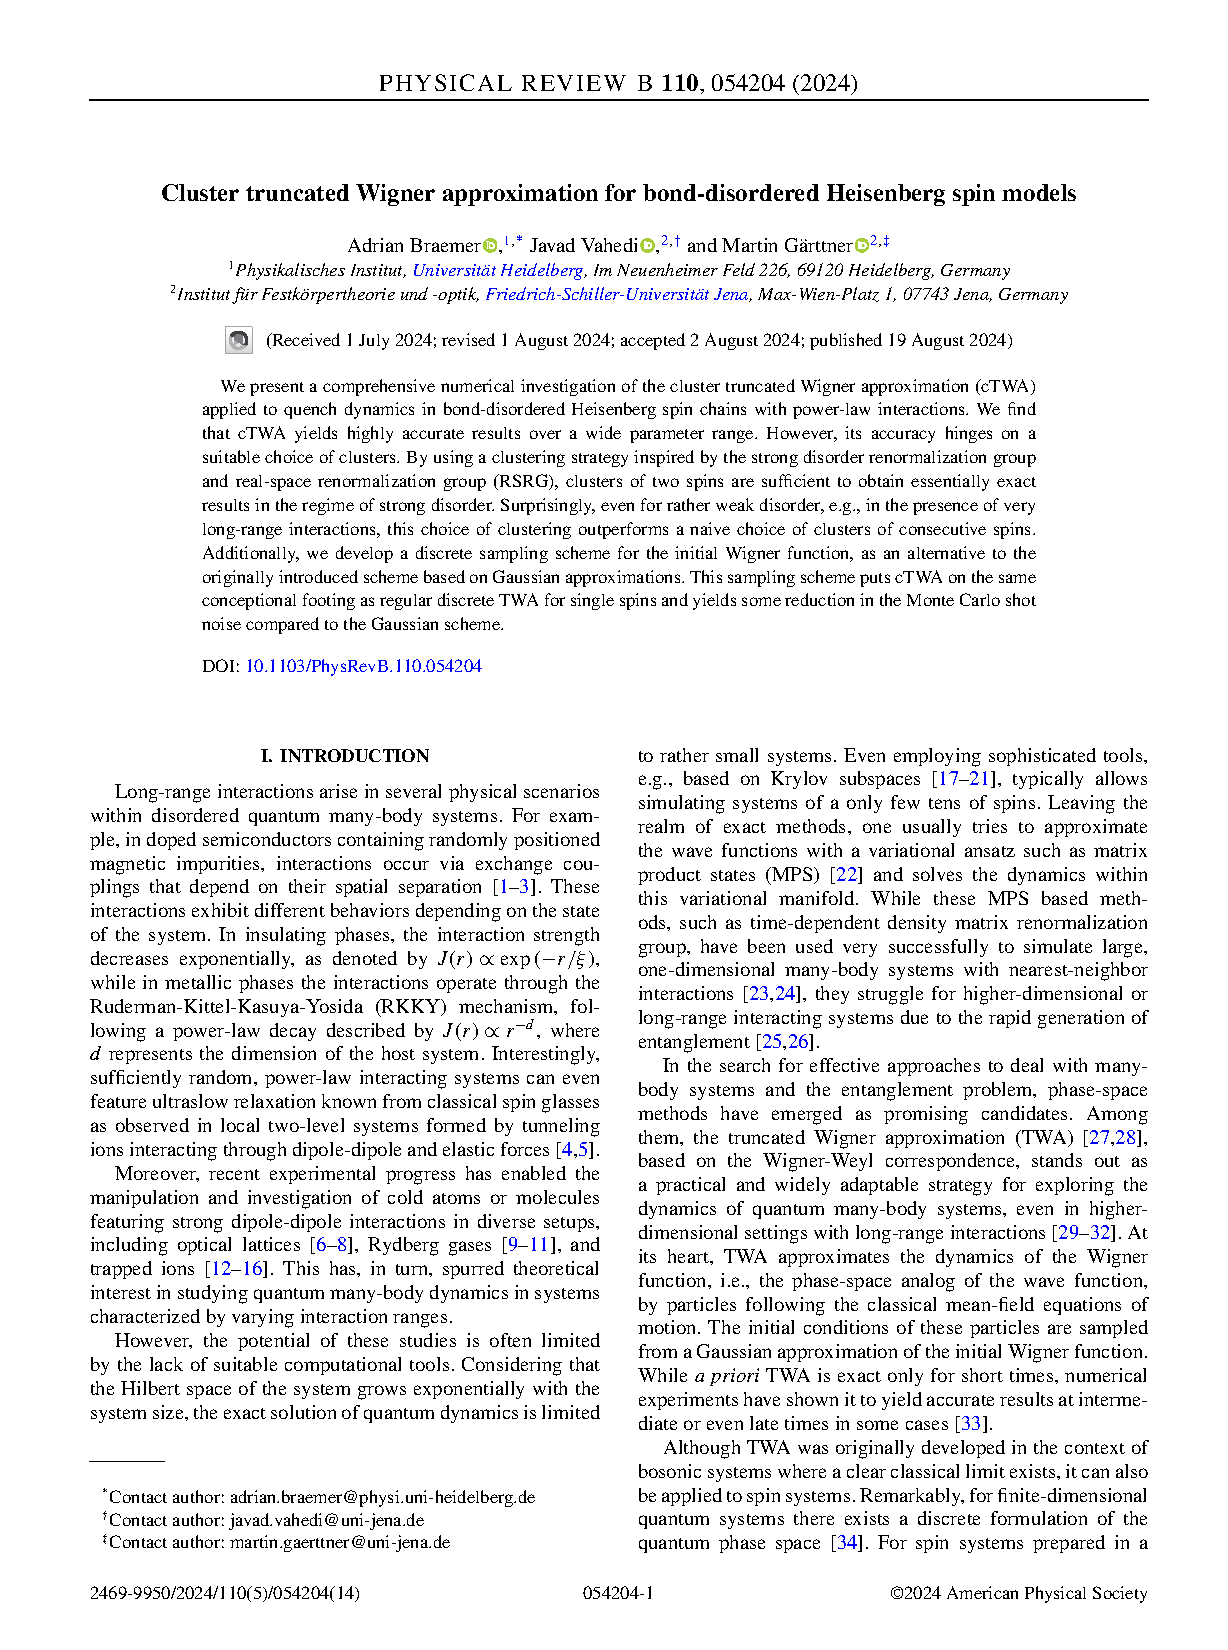
\includepdf[pages=-]{pub-Braemer2024-cTWA}